\documentclass[twoside]{book}

% Packages required by doxygen
\usepackage{fixltx2e}
\usepackage{calc}
\usepackage{doxygen}
\usepackage{graphicx}
\usepackage[utf8]{inputenc}
\usepackage{makeidx}
\usepackage{multicol}
\usepackage{multirow}
\PassOptionsToPackage{warn}{textcomp}
\usepackage{textcomp}
\usepackage[nointegrals]{wasysym}
\usepackage[table]{xcolor}

% Font selection
\usepackage[T1]{fontenc}
\usepackage{mathptmx}
\usepackage[scaled=.90]{helvet}
\usepackage{courier}
\usepackage{amssymb}
\usepackage{sectsty}
\renewcommand{\familydefault}{\sfdefault}
\allsectionsfont{%
  \fontseries{bc}\selectfont%
  \color{darkgray}%
}
\renewcommand{\DoxyLabelFont}{%
  \fontseries{bc}\selectfont%
  \color{darkgray}%
}
\newcommand{\+}{\discretionary{\mbox{\scriptsize$\hookleftarrow$}}{}{}}

% Page & text layout
\usepackage{geometry}
\geometry{%
  a4paper,%
  top=2.5cm,%
  bottom=2.5cm,%
  left=2.5cm,%
  right=2.5cm%
}
\tolerance=750
\hfuzz=15pt
\hbadness=750
\setlength{\emergencystretch}{15pt}
\setlength{\parindent}{0cm}
\setlength{\parskip}{0.2cm}
\makeatletter
\renewcommand{\paragraph}{%
  \@startsection{paragraph}{4}{0ex}{-1.0ex}{1.0ex}{%
    \normalfont\normalsize\bfseries\SS@parafont%
  }%
}
\renewcommand{\subparagraph}{%
  \@startsection{subparagraph}{5}{0ex}{-1.0ex}{1.0ex}{%
    \normalfont\normalsize\bfseries\SS@subparafont%
  }%
}
\makeatother

% Headers & footers
\usepackage{fancyhdr}
\pagestyle{fancyplain}
\fancyhead[LE]{\fancyplain{}{\bfseries\thepage}}
\fancyhead[CE]{\fancyplain{}{}}
\fancyhead[RE]{\fancyplain{}{\bfseries\leftmark}}
\fancyhead[LO]{\fancyplain{}{\bfseries\rightmark}}
\fancyhead[CO]{\fancyplain{}{}}
\fancyhead[RO]{\fancyplain{}{\bfseries\thepage}}
\fancyfoot[LE]{\fancyplain{}{}}
\fancyfoot[CE]{\fancyplain{}{}}
\fancyfoot[RE]{\fancyplain{}{\bfseries\scriptsize Generated on Mon Dec 1 2014 02\+:29\+:17 for My Project by Doxygen }}
\fancyfoot[LO]{\fancyplain{}{\bfseries\scriptsize Generated on Mon Dec 1 2014 02\+:29\+:17 for My Project by Doxygen }}
\fancyfoot[CO]{\fancyplain{}{}}
\fancyfoot[RO]{\fancyplain{}{}}
\renewcommand{\footrulewidth}{0.4pt}
\renewcommand{\chaptermark}[1]{%
  \markboth{#1}{}%
}
\renewcommand{\sectionmark}[1]{%
  \markright{\thesection\ #1}%
}

% Indices & bibliography
\usepackage{natbib}
\usepackage[titles]{tocloft}
\setcounter{tocdepth}{3}
\setcounter{secnumdepth}{5}
\makeindex

% Hyperlinks (required, but should be loaded last)
\usepackage{ifpdf}
\ifpdf
  \usepackage[pdftex,pagebackref=true]{hyperref}
\else
  \usepackage[ps2pdf,pagebackref=true]{hyperref}
\fi
\hypersetup{%
  colorlinks=true,%
  linkcolor=blue,%
  citecolor=blue,%
  unicode%
}

% Custom commands
\newcommand{\clearemptydoublepage}{%
  \newpage{\pagestyle{empty}\cleardoublepage}%
}


%===== C O N T E N T S =====

\begin{document}

% Titlepage & ToC
\hypersetup{pageanchor=false,
             bookmarks=true,
             bookmarksnumbered=true,
             pdfencoding=unicode
            }
\pagenumbering{roman}
\begin{titlepage}
\vspace*{7cm}
\begin{center}%
{\Large My Project }\\
\vspace*{1cm}
{\large Generated by Doxygen 1.8.8}\\
\vspace*{0.5cm}
{\small Mon Dec 1 2014 02:29:17}\\
\end{center}
\end{titlepage}
\clearemptydoublepage
\tableofcontents
\clearemptydoublepage
\pagenumbering{arabic}
\hypersetup{pageanchor=true}

%--- Begin generated contents ---
\chapter{Hierarchical Index}
\section{Class Hierarchy}
This inheritance list is sorted roughly, but not completely, alphabetically\+:\begin{DoxyCompactList}
\item \contentsline{section}{Queue$<$ Data\+Type $>$}{\pageref{class_queue}}{}
\begin{DoxyCompactList}
\item \contentsline{section}{Queue\+Array$<$ Data\+Type $>$}{\pageref{class_queue_array}}{}
\item \contentsline{section}{Queue\+Linked$<$ Data\+Type $>$}{\pageref{class_queue_linked}}{}
\end{DoxyCompactList}
\end{DoxyCompactList}

\chapter{Class Index}
\section{Class List}
Here are the classes, structs, unions and interfaces with brief descriptions\+:\begin{DoxyCompactList}
\item\contentsline{section}{\hyperlink{class_greater}{Greater$<$ Key\+Type $>$} }{\pageref{class_greater}}{}
\item\contentsline{section}{\hyperlink{class_heap}{Heap$<$ Data\+Type, Key\+Type, Comparator $>$} }{\pageref{class_heap}}{}
\item\contentsline{section}{\hyperlink{class_less}{Less$<$ Key\+Type $>$} }{\pageref{class_less}}{}
\item\contentsline{section}{\hyperlink{class_priority_queue}{Priority\+Queue$<$ Data\+Type, Key\+Type, Comparator $>$} }{\pageref{class_priority_queue}}{}
\item\contentsline{section}{\hyperlink{struct_task_data}{Task\+Data} }{\pageref{struct_task_data}}{}
\item\contentsline{section}{\hyperlink{class_test_data}{Test\+Data} }{\pageref{class_test_data}}{}
\item\contentsline{section}{\hyperlink{class_test_data_item}{Test\+Data\+Item$<$ Key\+Type $>$} }{\pageref{class_test_data_item}}{}
\end{DoxyCompactList}

\chapter{File Index}
\section{File List}
Here is a list of all documented files with brief descriptions\+:\begin{DoxyCompactList}
\item\contentsline{section}{\hyperlink{_b_s_tree_8cpp}{B\+S\+Tree.\+cpp} \\*This program will implement a Binary Search Tree }{\pageref{_b_s_tree_8cpp}}{}
\item\contentsline{section}{{\bfseries B\+S\+Tree.\+h} }{\pageref{_b_s_tree_8h}}{}
\item\contentsline{section}{\hyperlink{_hash_table_8cpp}{Hash\+Table.\+cpp} \\*This program will implement a Hash Table }{\pageref{_hash_table_8cpp}}{}
\item\contentsline{section}{{\bfseries Hash\+Table.\+h} }{\pageref{_hash_table_8h}}{}
\item\contentsline{section}{\hyperlink{login_8cpp}{login.\+cpp} \\*This program will implement the Exercise 1 of Lab 10 Hash Table }{\pageref{login_8cpp}}{}
\end{DoxyCompactList}

\chapter{Class Documentation}
\hypertarget{class_greater}{\section{Greater$<$ Key\+Type $>$ Class Template Reference}
\label{class_greater}\index{Greater$<$ Key\+Type $>$@{Greater$<$ Key\+Type $>$}}
}
\subsection*{Public Member Functions}
\begin{DoxyCompactItemize}
\item 
\hypertarget{class_greater_a79d9cb7121723ee9d65b11cb2fce0379}{bool {\bfseries operator()} (const Key\+Type \&a, const Key\+Type \&b) const }\label{class_greater_a79d9cb7121723ee9d65b11cb2fce0379}

\end{DoxyCompactItemize}


The documentation for this class was generated from the following file\+:\begin{DoxyCompactItemize}
\item 
test11.\+cpp\end{DoxyCompactItemize}

\hypertarget{class_heap}{\section{Heap$<$ Data\+Type, Key\+Type, Comparator $>$ Class Template Reference}
\label{class_heap}\index{Heap$<$ Data\+Type, Key\+Type, Comparator $>$@{Heap$<$ Data\+Type, Key\+Type, Comparator $>$}}
}
\subsection*{Public Member Functions}
\begin{DoxyCompactItemize}
\item 
\hyperlink{class_heap_ae17e34e3c86d88263a8fdf80b9ba78fc}{Heap} (int max\+Number=D\+E\+F\+A\+U\+L\+T\+\_\+\+M\+A\+X\+\_\+\+H\+E\+A\+P\+\_\+\+S\+I\+Z\+E)
\item 
\hyperlink{class_heap_a97e3b462be1c6af31d7519546bba8907}{Heap} (const \hyperlink{class_heap}{Heap} \&other)
\item 
\hyperlink{class_heap}{Heap} \& \hyperlink{class_heap_a5ed119341c39bcea1437321d4247dd40}{operator=} (const \hyperlink{class_heap}{Heap} \&other)
\item 
\hyperlink{class_heap_a555ade7891007de959bef0ee53e28767}{$\sim$\+Heap} ()
\item 
void \hyperlink{class_heap_aa68cf80454ab1b246fa723612805a91e}{insert} (const Data\+Type \&new\+Data\+Item)  throw ( logic\+\_\+error )
\item 
Data\+Type \hyperlink{class_heap_a4a18bfdacd897c45fc3da13f22b8930d}{remove} ()  throw ( logic\+\_\+error )
\item 
void \hyperlink{class_heap_a19a78c8eae2cf7c8253e34e54d86ed73}{clear} ()
\item 
bool \hyperlink{class_heap_ab8fa26d416ac0e27dfcbf18c54f8f73f}{is\+Empty} () const 
\item 
bool \hyperlink{class_heap_ac9111b884c74a376240e0155a788756e}{is\+Full} () const 
\item 
void \hyperlink{class_heap_a3ae1e1f27a145749c8b9f2da777cb8bc}{show\+Structure} () const 
\item 
void \hyperlink{class_heap_a4bdb1772ea92899de245d6cbd217d085}{write\+Levels} () const 
\end{DoxyCompactItemize}
\subsection*{Static Public Attributes}
\begin{DoxyCompactItemize}
\item 
\hypertarget{class_heap_a967c19732a20a72e8e824402ad6763c8}{static const int {\bfseries D\+E\+F\+A\+U\+L\+T\+\_\+\+M\+A\+X\+\_\+\+H\+E\+A\+P\+\_\+\+S\+I\+Z\+E} = 10}\label{class_heap_a967c19732a20a72e8e824402ad6763c8}

\end{DoxyCompactItemize}


\subsection{Constructor \& Destructor Documentation}
\hypertarget{class_heap_ae17e34e3c86d88263a8fdf80b9ba78fc}{\index{Heap@{Heap}!Heap@{Heap}}
\index{Heap@{Heap}!Heap@{Heap}}
\subsubsection[{Heap}]{\setlength{\rightskip}{0pt plus 5cm}template$<$typename Data\+Type , typename Key\+Type , typename Comparator $>$ {\bf Heap}$<$ Data\+Type, Key\+Type, Comparator $>$\+::{\bf Heap} (
\begin{DoxyParamCaption}
\item[{int}]{max\+Number = {\ttfamily DEFAULT\+\_\+MAX\+\_\+HEAP\+\_\+SIZE}}
\end{DoxyParamCaption}
)}}\label{class_heap_ae17e34e3c86d88263a8fdf80b9ba78fc}
Constructor for \hyperlink{class_heap}{Heap}. Creates an empty heap. Allocates enough memory for a heap containing max\+Number data items. Pseudocode\+: set max\+Size equal to max\+Number, allocate memory for data\+Items based on max\+Size, and set size to 0


\begin{DoxyParams}{Parameters}
{\em max\+Number} & \+: The maximum number of elements that can be in this heap \\
\hline
\end{DoxyParams}
\begin{DoxyReturn}{Returns}
None 
\end{DoxyReturn}
\begin{DoxyPrecond}{Precondition}
None 
\end{DoxyPrecond}
\begin{DoxyPostcond}{Postcondition}
This heap will have a max\+Size and size defined, and our heap will be initialized 
\end{DoxyPostcond}
\hypertarget{class_heap_a97e3b462be1c6af31d7519546bba8907}{\index{Heap@{Heap}!Heap@{Heap}}
\index{Heap@{Heap}!Heap@{Heap}}
\subsubsection[{Heap}]{\setlength{\rightskip}{0pt plus 5cm}template$<$typename Data\+Type , typename Key\+Type , typename Comparator $>$ {\bf Heap}$<$ Data\+Type, Key\+Type, Comparator $>$\+::{\bf Heap} (
\begin{DoxyParamCaption}
\item[{const {\bf Heap}$<$ Data\+Type, Key\+Type, Comparator $>$ \&}]{other}
\end{DoxyParamCaption}
)}}\label{class_heap_a97e3b462be1c6af31d7519546bba8907}
Copy constructor for \hyperlink{class_heap}{Heap}. Initializes the object to be an equivalent copy of other. Pseudocode\+:
\begin{DoxyEnumerate}
\item Set max\+Size equal to other's max size, size to other's max size, allocate memory to data\+Items based on max\+Size, and use a loop to traverse through our elements to set them equal to other's elements.
\end{DoxyEnumerate}


\begin{DoxyParams}{Parameters}
{\em } & return \\
\hline
\end{DoxyParams}
\begin{DoxyPrecond}{Precondition}
None 
\end{DoxyPrecond}
\begin{DoxyPostcond}{Postcondition}
This heap will be equal to other 
\end{DoxyPostcond}
\hypertarget{class_heap_a555ade7891007de959bef0ee53e28767}{\index{Heap@{Heap}!````~Heap@{$\sim$\+Heap}}
\index{````~Heap@{$\sim$\+Heap}!Heap@{Heap}}
\subsubsection[{$\sim$\+Heap}]{\setlength{\rightskip}{0pt plus 5cm}template$<$typename Data\+Type , typename Key\+Type , typename Comparator $>$ {\bf Heap}$<$ Data\+Type, Key\+Type, Comparator $>$\+::$\sim${\bf Heap} (
\begin{DoxyParamCaption}
{}
\end{DoxyParamCaption}
)}}\label{class_heap_a555ade7891007de959bef0ee53e28767}
Destructor for \hyperlink{class_heap}{Heap}. Deallocates (frees) the memory used to store the heap. Pseudocode\+: Call the clear method


\begin{DoxyParams}{Parameters}
{\em None} & \\
\hline
\end{DoxyParams}
\begin{DoxyReturn}{Returns}
None 
\end{DoxyReturn}
\begin{DoxyPrecond}{Precondition}
None 
\end{DoxyPrecond}
\begin{DoxyPostcond}{Postcondition}
All memory being used by this heap will be deallocated 
\end{DoxyPostcond}


\subsection{Member Function Documentation}
\hypertarget{class_heap_a19a78c8eae2cf7c8253e34e54d86ed73}{\index{Heap@{Heap}!clear@{clear}}
\index{clear@{clear}!Heap@{Heap}}
\subsubsection[{clear}]{\setlength{\rightskip}{0pt plus 5cm}template$<$typename Data\+Type , typename Key\+Type , typename Comparator $>$ void {\bf Heap}$<$ Data\+Type, Key\+Type, Comparator $>$\+::clear (
\begin{DoxyParamCaption}
{}
\end{DoxyParamCaption}
)}}\label{class_heap_a19a78c8eae2cf7c8253e34e54d86ed73}
Removes all the data items in the heap. Pseudocode\+: delete the array. Set size to 0.


\begin{DoxyParams}{Parameters}
{\em None} & \\
\hline
\end{DoxyParams}
\begin{DoxyReturn}{Returns}
None 
\end{DoxyReturn}
\begin{DoxyPrecond}{Precondition}
None 
\end{DoxyPrecond}
\begin{DoxyPostcond}{Postcondition}
Size will be set to 0 and all memory deallocated from the heap 
\end{DoxyPostcond}
\hypertarget{class_heap_aa68cf80454ab1b246fa723612805a91e}{\index{Heap@{Heap}!insert@{insert}}
\index{insert@{insert}!Heap@{Heap}}
\subsubsection[{insert}]{\setlength{\rightskip}{0pt plus 5cm}template$<$typename Data\+Type, typename Key\+Type , typename Comparator $>$ void {\bf Heap}$<$ Data\+Type, Key\+Type, Comparator $>$\+::insert (
\begin{DoxyParamCaption}
\item[{const Data\+Type \&}]{new\+Data\+Item}
\end{DoxyParamCaption}
) throw  logic\+\_\+error) }}\label{class_heap_aa68cf80454ab1b246fa723612805a91e}
Inserts new\+Data\+Item into the heap. Inserts this data item as the bottom rightmost data item in the heap and moves it upward until the properties that define a heap are restored. Pseudocode\+:
\begin{DoxyEnumerate}
\item Check if full. If so, throw logic error. Otherwise, go to 2.
\item Set data\+Items\mbox{[}size\mbox{]} to parameter passed in
\item Increment size (so that the index we just set is now valid within the heap)
\item Call the reprioritize method
\end{DoxyEnumerate}


\begin{DoxyParams}{Parameters}
{\em new\+Data\+Item} & \+: new item to be inserted into the list \\
\hline
\end{DoxyParams}
\begin{DoxyReturn}{Returns}
None 
\end{DoxyReturn}
\begin{DoxyPrecond}{Precondition}
\hyperlink{class_heap}{Heap} is not full 
\end{DoxyPrecond}
\begin{DoxyPostcond}{Postcondition}
The new\+Data\+Item will be inserted, and the rest of the heap will be sorted based on this new insertion 
\end{DoxyPostcond}

\begin{DoxyExceptions}{Exceptions}
{\em logic\+\_\+error} & \+: Throws a logic error if the heap is full \\
\hline
\end{DoxyExceptions}
\hypertarget{class_heap_ab8fa26d416ac0e27dfcbf18c54f8f73f}{\index{Heap@{Heap}!is\+Empty@{is\+Empty}}
\index{is\+Empty@{is\+Empty}!Heap@{Heap}}
\subsubsection[{is\+Empty}]{\setlength{\rightskip}{0pt plus 5cm}template$<$typename Data\+Type , typename Key\+Type , typename Comparator $>$ bool {\bf Heap}$<$ Data\+Type, Key\+Type, Comparator $>$\+::is\+Empty (
\begin{DoxyParamCaption}
{}
\end{DoxyParamCaption}
) const}}\label{class_heap_ab8fa26d416ac0e27dfcbf18c54f8f73f}
Returns true if the heap is empty. Otherwise, returns false. Pseudocode\+: return size == 0


\begin{DoxyParams}{Parameters}
{\em None} & \\
\hline
\end{DoxyParams}
\begin{DoxyReturn}{Returns}
bool \+: true if heap is empty, false otherwise 
\end{DoxyReturn}
\begin{DoxyPrecond}{Precondition}
None 
\end{DoxyPrecond}
\begin{DoxyPostcond}{Postcondition}
The elements of the heap will not be changed. 
\end{DoxyPostcond}
\hypertarget{class_heap_ac9111b884c74a376240e0155a788756e}{\index{Heap@{Heap}!is\+Full@{is\+Full}}
\index{is\+Full@{is\+Full}!Heap@{Heap}}
\subsubsection[{is\+Full}]{\setlength{\rightskip}{0pt plus 5cm}template$<$typename Data\+Type , typename Key\+Type , typename Comparator $>$ bool {\bf Heap}$<$ Data\+Type, Key\+Type, Comparator $>$\+::is\+Full (
\begin{DoxyParamCaption}
{}
\end{DoxyParamCaption}
) const}}\label{class_heap_ac9111b884c74a376240e0155a788756e}
Returns true if the heap is full. Otherwise, returns false. Pseudocode\+: return size == max\+Size


\begin{DoxyParams}{Parameters}
{\em None} & \\
\hline
\end{DoxyParams}
\begin{DoxyReturn}{Returns}
bool \+: True if heap is full, false otherwise 
\end{DoxyReturn}
\begin{DoxyPrecond}{Precondition}
None 
\end{DoxyPrecond}
\begin{DoxyPostcond}{Postcondition}
The elements of the heap will not be changed. 
\end{DoxyPostcond}
\hypertarget{class_heap_a5ed119341c39bcea1437321d4247dd40}{\index{Heap@{Heap}!operator=@{operator=}}
\index{operator=@{operator=}!Heap@{Heap}}
\subsubsection[{operator=}]{\setlength{\rightskip}{0pt plus 5cm}template$<$typename Data\+Type , typename Key\+Type , typename Comparator $>$ {\bf Heap}$<$ Data\+Type, Key\+Type, Comparator $>$ \& {\bf Heap}$<$ Data\+Type, Key\+Type, Comparator $>$\+::operator= (
\begin{DoxyParamCaption}
\item[{const {\bf Heap}$<$ Data\+Type, Key\+Type, Comparator $>$ \&}]{other}
\end{DoxyParamCaption}
)}}\label{class_heap_a5ed119341c39bcea1437321d4247dd40}
Overloaded assignment operator for \hyperlink{class_heap}{Heap}. Sets the heap to be equivalent to the other \hyperlink{class_heap}{Heap} and returns a reference to this object. Pseudocode\+:
\begin{DoxyEnumerate}
\item Check if this already equals the other. If it does, stop right there and just return
\item Otherwise, clear the heap.
\item Set max\+Size equal to other's max size, size to other's max size, allocate memory to data\+Items based on max\+Size, and use a loop to traverse through our elements to set them equal to other's elements.
\item Returns this.
\end{DoxyEnumerate}


\begin{DoxyParams}{Parameters}
{\em other} & \+: Another heap of which this heap will become a copy of \\
\hline
\end{DoxyParams}
\begin{DoxyReturn}{Returns}
\hyperlink{class_heap}{Heap} \+: This 
\end{DoxyReturn}
\begin{DoxyPrecond}{Precondition}
None 
\end{DoxyPrecond}
\begin{DoxyPostcond}{Postcondition}
This heap will be equal to other 
\end{DoxyPostcond}
\hypertarget{class_heap_a4a18bfdacd897c45fc3da13f22b8930d}{\index{Heap@{Heap}!remove@{remove}}
\index{remove@{remove}!Heap@{Heap}}
\subsubsection[{remove}]{\setlength{\rightskip}{0pt plus 5cm}template$<$typename Data\+Type , typename Key\+Type , typename Comparator $>$ Data\+Type {\bf Heap}$<$ Data\+Type, Key\+Type, Comparator $>$\+::remove (
\begin{DoxyParamCaption}
{}
\end{DoxyParamCaption}
) throw  logic\+\_\+error) }}\label{class_heap_a4a18bfdacd897c45fc3da13f22b8930d}
Removes the data item with the highest priority (the root) from the heap and returns it. Replaces the root data item with the bottom rightmost data item and moves this data item downward until the properties that define a heap are restored. Pseudocode\+:
\begin{DoxyEnumerate}
\item If empty, throw logic error. Else go to 2.
\item Swap root with last elements
\item Decrement size
\item Call reprioritize method
\item Return item at size (that item is technically out of bounds of our heap, but it still exists in memory so utilize this)
\end{DoxyEnumerate}


\begin{DoxyParams}{Parameters}
{\em None} & \\
\hline
\end{DoxyParams}
\begin{DoxyReturn}{Returns}
Data\+Type Highest priority item / root 
\end{DoxyReturn}
\begin{DoxyPrecond}{Precondition}
\hyperlink{class_heap}{Heap} is not empty 
\end{DoxyPrecond}
\begin{DoxyPostcond}{Postcondition}
Root will have been removed, and replaced, and everything will be sorted 
\end{DoxyPostcond}

\begin{DoxyExceptions}{Exceptions}
{\em logic\+\_\+error} & \+: Throws an error if the heap is empty \\
\hline
\end{DoxyExceptions}
\hypertarget{class_heap_a3ae1e1f27a145749c8b9f2da777cb8bc}{\index{Heap@{Heap}!show\+Structure@{show\+Structure}}
\index{show\+Structure@{show\+Structure}!Heap@{Heap}}
\subsubsection[{show\+Structure}]{\setlength{\rightskip}{0pt plus 5cm}template$<$typename Data\+Type , typename Key\+Type , typename Comparator $>$ void {\bf Heap}$<$ Data\+Type, Key\+Type, Comparator $>$\+::show\+Structure (
\begin{DoxyParamCaption}
{}
\end{DoxyParamCaption}
) const}}\label{class_heap_a3ae1e1f27a145749c8b9f2da777cb8bc}
Outputs the priorities of the data items in the heap in both array and tree form. The tree is output with its branches oriented from left (root) to right (leaves) -\/ that is, the tree is output rotated counterclockwise ninety degrees from its conventional orientation. If the heap is empty, outputs \char`\"{}\+Empty heap\char`\"{}. Note that this operation is intended for testing/debugging purposes only.


\begin{DoxyParams}{Parameters}
{\em None} & \\
\hline
\end{DoxyParams}
\begin{DoxyReturn}{Returns}
None 
\end{DoxyReturn}
\begin{DoxyPrecond}{Precondition}
None 
\end{DoxyPrecond}
\begin{DoxyPostcond}{Postcondition}
The contents of this heap will not be changed. 
\end{DoxyPostcond}
\hypertarget{class_heap_a4bdb1772ea92899de245d6cbd217d085}{\index{Heap@{Heap}!write\+Levels@{write\+Levels}}
\index{write\+Levels@{write\+Levels}!Heap@{Heap}}
\subsubsection[{write\+Levels}]{\setlength{\rightskip}{0pt plus 5cm}template$<$typename Data\+Type , typename Key\+Type , typename Comparator $>$ void {\bf Heap}$<$ Data\+Type, Key\+Type, Comparator $>$\+::write\+Levels (
\begin{DoxyParamCaption}
{}
\end{DoxyParamCaption}
) const}}\label{class_heap_a4bdb1772ea92899de245d6cbd217d085}
Writes each level of the tree. Pseudocode\+:
\begin{DoxyEnumerate}
\item Use loop to go through entire tree (condition being that the \char`\"{}current\+Node\char`\"{} is less than size).
\item Check if the current\+Node index is less than the index of the next level.
\item If it is, output the current\+Node and increment current\+Node.
\item Otherwise, output an endl and increase the next\+Level to the appropriate length (2$\ast$current\+Node + 1)
\end{DoxyEnumerate}


\begin{DoxyParams}{Parameters}
{\em None} & \\
\hline
\end{DoxyParams}
\begin{DoxyReturn}{Returns}
None 
\end{DoxyReturn}
\begin{DoxyPrecond}{Precondition}
None 
\end{DoxyPrecond}
\begin{DoxyPostcond}{Postcondition}
None 
\end{DoxyPostcond}


The documentation for this class was generated from the following files\+:\begin{DoxyCompactItemize}
\item 
Heap.\+h\item 
\hyperlink{_heap_8cpp}{Heap.\+cpp}\item 
show11.\+cpp\end{DoxyCompactItemize}

\hypertarget{class_less}{\section{Less$<$ Key\+Type $>$ Class Template Reference}
\label{class_less}\index{Less$<$ Key\+Type $>$@{Less$<$ Key\+Type $>$}}
}
\subsection*{Public Member Functions}
\begin{DoxyCompactItemize}
\item 
\hypertarget{class_less_afee76a5248eb9c6c8fd1f005360d44d5}{bool {\bfseries operator()} (const Key\+Type \&a, const Key\+Type \&b) const }\label{class_less_afee76a5248eb9c6c8fd1f005360d44d5}

\end{DoxyCompactItemize}


The documentation for this class was generated from the following file\+:\begin{DoxyCompactItemize}
\item 
Heap.\+h\end{DoxyCompactItemize}

\hypertarget{class_priority_queue}{\section{Priority\+Queue$<$ Data\+Type, Key\+Type, Comparator $>$ Class Template Reference}
\label{class_priority_queue}\index{Priority\+Queue$<$ Data\+Type, Key\+Type, Comparator $>$@{Priority\+Queue$<$ Data\+Type, Key\+Type, Comparator $>$}}
}
Inheritance diagram for Priority\+Queue$<$ Data\+Type, Key\+Type, Comparator $>$\+:\begin{figure}[H]
\begin{center}
\leavevmode
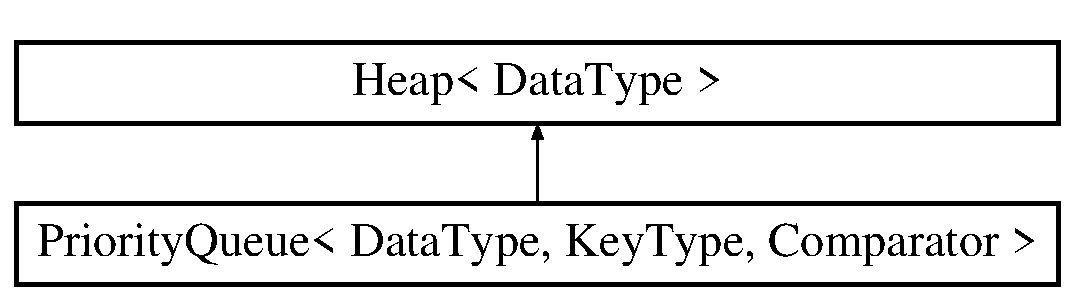
\includegraphics[height=2.000000cm]{class_priority_queue}
\end{center}
\end{figure}
\subsection*{Public Member Functions}
\begin{DoxyCompactItemize}
\item 
\hyperlink{class_priority_queue_a47de2a46cff1d6a6ed30a99c94dc1b14}{Priority\+Queue} (int max\+Number=def\+Max\+Queue\+Size)
\item 
\hyperlink{class_priority_queue_a7d959dc823b18c647aa0ee4a80f27881}{$\sim$\+Priority\+Queue} ()
\item 
void \hyperlink{class_priority_queue_a61f3339cf0e87c67ed004f8eff0a1bfa}{enqueue} (const Data\+Type \&new\+Data\+Item)
\item 
Data\+Type \hyperlink{class_priority_queue_a5bc758e313d6244e672ea6e81d695a46}{dequeue} ()
\end{DoxyCompactItemize}
\subsection*{Additional Inherited Members}


\subsection{Constructor \& Destructor Documentation}
\hypertarget{class_priority_queue_a47de2a46cff1d6a6ed30a99c94dc1b14}{\index{Priority\+Queue@{Priority\+Queue}!Priority\+Queue@{Priority\+Queue}}
\index{Priority\+Queue@{Priority\+Queue}!Priority\+Queue@{Priority\+Queue}}
\subsubsection[{Priority\+Queue}]{\setlength{\rightskip}{0pt plus 5cm}template$<$typename Data\+Type , typename Key\+Type , typename Comparator $>$ {\bf Priority\+Queue}$<$ Data\+Type, Key\+Type, Comparator $>$\+::{\bf Priority\+Queue} (
\begin{DoxyParamCaption}
\item[{int}]{max\+Number = {\ttfamily defMaxQueueSize}}
\end{DoxyParamCaption}
)}}\label{class_priority_queue_a47de2a46cff1d6a6ed30a99c94dc1b14}
Constructor for \hyperlink{class_priority_queue}{Priority\+Queue}. Calls constructor for heap. Set max\+Number of items this Priority\+Heap can hold.


\begin{DoxyParams}{Parameters}
{\em max\+Number} & \+: maximum number of items allowed in this heap. \\
\hline
\end{DoxyParams}
\begin{DoxyReturn}{Returns}
None 
\end{DoxyReturn}
\begin{DoxyPrecond}{Precondition}
None 
\end{DoxyPrecond}
\begin{DoxyPostcond}{Postcondition}
This Priority\+Heap will be initialized. 
\end{DoxyPostcond}
\hypertarget{class_priority_queue_a7d959dc823b18c647aa0ee4a80f27881}{\index{Priority\+Queue@{Priority\+Queue}!````~Priority\+Queue@{$\sim$\+Priority\+Queue}}
\index{````~Priority\+Queue@{$\sim$\+Priority\+Queue}!Priority\+Queue@{Priority\+Queue}}
\subsubsection[{$\sim$\+Priority\+Queue}]{\setlength{\rightskip}{0pt plus 5cm}template$<$typename Data\+Type , typename Key\+Type , typename Comparator $>$ {\bf Priority\+Queue}$<$ Data\+Type, Key\+Type, Comparator $>$\+::$\sim${\bf Priority\+Queue} (
\begin{DoxyParamCaption}
{}
\end{DoxyParamCaption}
)}}\label{class_priority_queue_a7d959dc823b18c647aa0ee4a80f27881}
Destructor for Priority\+Heap. Deallocates all memory in this heap. Calls \hyperlink{class_heap}{Heap} clear method.


\begin{DoxyParams}{Parameters}
{\em None} & \\
\hline
\end{DoxyParams}
\begin{DoxyReturn}{Returns}
None 
\end{DoxyReturn}
\begin{DoxyPrecond}{Precondition}
None 
\end{DoxyPrecond}
\begin{DoxyPostcond}{Postcondition}
All memory of this heap will be deallocated. 
\end{DoxyPostcond}


\subsection{Member Function Documentation}
\hypertarget{class_priority_queue_a5bc758e313d6244e672ea6e81d695a46}{\index{Priority\+Queue@{Priority\+Queue}!dequeue@{dequeue}}
\index{dequeue@{dequeue}!Priority\+Queue@{Priority\+Queue}}
\subsubsection[{dequeue}]{\setlength{\rightskip}{0pt plus 5cm}template$<$typename Data\+Type , typename Key\+Type , typename Comparator $>$ Data\+Type {\bf Priority\+Queue}$<$ Data\+Type, Key\+Type, Comparator $>$\+::dequeue (
\begin{DoxyParamCaption}
{}
\end{DoxyParamCaption}
)}}\label{class_priority_queue_a5bc758e313d6244e672ea6e81d695a46}
Removes highest priority item in the Priority\+Heap. Uses base heap's remove method.


\begin{DoxyParams}{Parameters}
{\em None} & \\
\hline
\end{DoxyParams}
\begin{DoxyReturn}{Returns}
Data\+Type \+: highest priority item that was removed from the Priority\+Heap 
\end{DoxyReturn}
\begin{DoxyPrecond}{Precondition}
None 
\end{DoxyPrecond}
\begin{DoxyPostcond}{Postcondition}
H\+Ighest priority item will be removed from the Priority\+Heap. 
\end{DoxyPostcond}
\hypertarget{class_priority_queue_a61f3339cf0e87c67ed004f8eff0a1bfa}{\index{Priority\+Queue@{Priority\+Queue}!enqueue@{enqueue}}
\index{enqueue@{enqueue}!Priority\+Queue@{Priority\+Queue}}
\subsubsection[{enqueue}]{\setlength{\rightskip}{0pt plus 5cm}template$<$typename Data\+Type , typename Key\+Type , typename Comparator $>$ void {\bf Priority\+Queue}$<$ Data\+Type, Key\+Type, Comparator $>$\+::enqueue (
\begin{DoxyParamCaption}
\item[{const Data\+Type \&}]{new\+Data\+Item}
\end{DoxyParamCaption}
)}}\label{class_priority_queue_a61f3339cf0e87c67ed004f8eff0a1bfa}
Enqueues an item into the \hyperlink{class_priority_queue}{Priority\+Queue}. Uses heap insert method.


\begin{DoxyParams}{Parameters}
{\em new\+Data\+Item} & \+: New item to insert into the Priority\+Heap. \\
\hline
\end{DoxyParams}
\begin{DoxyReturn}{Returns}
None 
\end{DoxyReturn}
\begin{DoxyPrecond}{Precondition}
None 
\end{DoxyPrecond}
\begin{DoxyPostcond}{Postcondition}
Item will be inserted into the heap. 
\end{DoxyPostcond}


The documentation for this class was generated from the following files\+:\begin{DoxyCompactItemize}
\item 
Priority\+Queue.\+h\item 
\hyperlink{_priority_queue_8cpp}{Priority\+Queue.\+cpp}\end{DoxyCompactItemize}

\hypertarget{struct_task_data}{\section{Task\+Data Struct Reference}
\label{struct_task_data}\index{Task\+Data@{Task\+Data}}
}
\subsection*{Public Member Functions}
\begin{DoxyCompactItemize}
\item 
\hypertarget{struct_task_data_a58cbe6eec8a86be7b827561a2f4b49c1}{int {\bfseries get\+Priority} () const }\label{struct_task_data_a58cbe6eec8a86be7b827561a2f4b49c1}

\item 
\hypertarget{struct_task_data_a58cbe6eec8a86be7b827561a2f4b49c1}{int {\bfseries get\+Priority} () const }\label{struct_task_data_a58cbe6eec8a86be7b827561a2f4b49c1}

\end{DoxyCompactItemize}
\subsection*{Public Attributes}
\begin{DoxyCompactItemize}
\item 
\hypertarget{struct_task_data_a9d8b606897eb428a62d816b71312e1b7}{int {\bfseries priority}}\label{struct_task_data_a9d8b606897eb428a62d816b71312e1b7}

\item 
\hypertarget{struct_task_data_a126fafee3369b6a2d8734f4e46c670bc}{int {\bfseries arrived}}\label{struct_task_data_a126fafee3369b6a2d8734f4e46c670bc}

\end{DoxyCompactItemize}


The documentation for this struct was generated from the following files\+:\begin{DoxyCompactItemize}
\item 
\hyperlink{ossim_8cpp}{ossim.\+cpp}\item 
ossim.\+cs\end{DoxyCompactItemize}

\hypertarget{class_test_data}{\section{Test\+Data Class Reference}
\label{class_test_data}\index{Test\+Data@{Test\+Data}}
}
\subsection*{Public Member Functions}
\begin{DoxyCompactItemize}
\item 
\hypertarget{class_test_data_a72cb0d5febcf77e8a6dd494fa6dff411}{void {\bfseries set\+Key} (const string \&new\+Key)}\label{class_test_data_a72cb0d5febcf77e8a6dd494fa6dff411}

\item 
\hypertarget{class_test_data_ac7fe71dc8c3eda2242e443d22523e286}{void {\bfseries set\+Value} (const string \&new\+Value)}\label{class_test_data_ac7fe71dc8c3eda2242e443d22523e286}

\item 
\hypertarget{class_test_data_ae20d0a4c5fba891d728c68ac4ec79654}{string {\bfseries get\+Key} () const }\label{class_test_data_ae20d0a4c5fba891d728c68ac4ec79654}

\item 
\hypertarget{class_test_data_af33e667b6962f8a351f7a660a1a24c5e}{string {\bfseries get\+Value} () const }\label{class_test_data_af33e667b6962f8a351f7a660a1a24c5e}

\item 
\hypertarget{class_test_data_a72cb0d5febcf77e8a6dd494fa6dff411}{void {\bfseries set\+Key} (const string \&new\+Key)}\label{class_test_data_a72cb0d5febcf77e8a6dd494fa6dff411}

\item 
\hypertarget{class_test_data_ae20d0a4c5fba891d728c68ac4ec79654}{string {\bfseries get\+Key} () const }\label{class_test_data_ae20d0a4c5fba891d728c68ac4ec79654}

\item 
\hypertarget{class_test_data_af33e667b6962f8a351f7a660a1a24c5e}{int {\bfseries get\+Value} () const }\label{class_test_data_af33e667b6962f8a351f7a660a1a24c5e}

\end{DoxyCompactItemize}
\subsection*{Static Public Member Functions}
\begin{DoxyCompactItemize}
\item 
\hypertarget{class_test_data_a55f0e2851aa330be9921303107982f98}{static unsigned int {\bfseries hash} (const string \&str)}\label{class_test_data_a55f0e2851aa330be9921303107982f98}

\item 
\hypertarget{class_test_data_ac38bf2161ad472cfa80703a87e7eda8a}{static unsigned int {\bfseries hash} (const string \&str)}\label{class_test_data_ac38bf2161ad472cfa80703a87e7eda8a}

\end{DoxyCompactItemize}


The documentation for this class was generated from the following files\+:\begin{DoxyCompactItemize}
\item 
\hyperlink{login_8cpp}{login.\+cpp}\item 
test10.\+cpp\end{DoxyCompactItemize}

\hypertarget{class_test_data_item}{\section{Test\+Data\+Item$<$ Key\+Type $>$ Class Template Reference}
\label{class_test_data_item}\index{Test\+Data\+Item$<$ Key\+Type $>$@{Test\+Data\+Item$<$ Key\+Type $>$}}
}
\subsection*{Public Member Functions}
\begin{DoxyCompactItemize}
\item 
\hypertarget{class_test_data_item_a84667429c081b1dbb212956c88011216}{void {\bfseries set\+Priority} (Key\+Type new\+Pty)}\label{class_test_data_item_a84667429c081b1dbb212956c88011216}

\item 
\hypertarget{class_test_data_item_ac1632213d959555ec8f5aee8a1505d72}{Key\+Type {\bfseries get\+Priority} () const }\label{class_test_data_item_ac1632213d959555ec8f5aee8a1505d72}

\end{DoxyCompactItemize}


The documentation for this class was generated from the following file\+:\begin{DoxyCompactItemize}
\item 
test11.\+cpp\end{DoxyCompactItemize}

\chapter{File Documentation}
\hypertarget{_heap_8cpp}{\section{Heap.\+cpp File Reference}
\label{_heap_8cpp}\index{Heap.\+cpp@{Heap.\+cpp}}
}


This program will implement a \hyperlink{class_heap}{Heap}.  


{\ttfamily \#include \char`\"{}Heap.\+h\char`\"{}}\\*


\subsection{Detailed Description}
This program will implement a \hyperlink{class_heap}{Heap}. 

\begin{DoxyAuthor}{Author}
Tim Kwist 
\end{DoxyAuthor}
\begin{DoxyVersion}{Version}
1.\+0
\end{DoxyVersion}
The specifications of this program are defined by C++ Data Structures\+: A Laboratory Course (3rd edition) by Brandle, J\+Geisler, Roberge, Whittington, lab 11. \begin{DoxyDate}{Date}
Wednesday, November 5, 2014 
\end{DoxyDate}

\hypertarget{ossim_8cpp}{\section{ossim.\+cpp File Reference}
\label{ossim_8cpp}\index{ossim.\+cpp@{ossim.\+cpp}}
}


This program will implement an operating system task scheduling system.  


{\ttfamily \#include $<$iostream$>$}\\*
{\ttfamily \#include $<$cstdlib$>$}\\*
{\ttfamily \#include \char`\"{}Priority\+Queue.\+cpp\char`\"{}}\\*
\subsection*{Classes}
\begin{DoxyCompactItemize}
\item 
struct \hyperlink{struct_task_data}{Task\+Data}
\end{DoxyCompactItemize}
\subsection*{Functions}
\begin{DoxyCompactItemize}
\item 
int \hyperlink{ossim_8cpp_ae66f6b31b5ad750f1fe042a706a4e3d4}{main} ()
\end{DoxyCompactItemize}


\subsection{Detailed Description}
This program will implement an operating system task scheduling system. 

\begin{DoxyAuthor}{Author}
Tim Kwist 
\end{DoxyAuthor}
\begin{DoxyVersion}{Version}
1.\+0
\end{DoxyVersion}
The specifications of this program are defined by C++ Data Structures\+: A Laboratory Course (3rd edition) by Brandle, J\+Geisler, Roberge, Whittington, lab 11. \begin{DoxyDate}{Date}
Wednesday, November 5, 2014 
\end{DoxyDate}


\subsection{Function Documentation}
\hypertarget{ossim_8cpp_ae66f6b31b5ad750f1fe042a706a4e3d4}{\index{ossim.\+cpp@{ossim.\+cpp}!main@{main}}
\index{main@{main}!ossim.\+cpp@{ossim.\+cpp}}
\subsubsection[{main}]{\setlength{\rightskip}{0pt plus 5cm}int main (
\begin{DoxyParamCaption}
{}
\end{DoxyParamCaption}
)}}\label{ossim_8cpp_ae66f6b31b5ad750f1fe042a706a4e3d4}
Programming Exercise \#1 for Lab 11. (Shell) Operating system task scheduling simulation Pseudocode\+:
\begin{DoxyEnumerate}
\item Get number of priority levels
\item Get length of time to run the simulator
\item Run loop for length of time to run the simulator. 3a. Dequeue item in \hyperlink{class_priority_queue}{Priority\+Queue} if it exists. Output the item dequeue'd. 3b. Determine number of items to add to the list based on a random number (50\% no items, 25\% 1 item, 25\% 2 items) 3c. Insert previously determined number of items into \hyperlink{class_priority_queue}{Priority\+Queue}.
\end{DoxyEnumerate}


\begin{DoxyParams}{Parameters}
{\em None} & \\
\hline
\end{DoxyParams}
\begin{DoxyReturn}{Returns}
int \+: default return for main function 
\end{DoxyReturn}
\begin{DoxyPrecond}{Precondition}
None 
\end{DoxyPrecond}
\begin{DoxyPostcond}{Postcondition}
None 
\end{DoxyPostcond}

\hypertarget{_priority_queue_8cpp}{\section{Priority\+Queue.\+cpp File Reference}
\label{_priority_queue_8cpp}\index{Priority\+Queue.\+cpp@{Priority\+Queue.\+cpp}}
}


This program will implement a \hyperlink{class_priority_queue}{Priority\+Queue}.  


{\ttfamily \#include \char`\"{}Priority\+Queue.\+h\char`\"{}}\\*


\subsection{Detailed Description}
This program will implement a \hyperlink{class_priority_queue}{Priority\+Queue}. 

\begin{DoxyAuthor}{Author}
Tim Kwist 
\end{DoxyAuthor}
\begin{DoxyVersion}{Version}
1.\+0
\end{DoxyVersion}
The specifications of this program are defined by C++ Data Structures\+: A Laboratory Course (3rd edition) by Brandle, J\+Geisler, Roberge, Whittington, lab 11. \begin{DoxyDate}{Date}
Wednesday, November 5, 2014 
\end{DoxyDate}

%--- End generated contents ---

% Index
\newpage
\phantomsection
\addcontentsline{toc}{chapter}{Index}
\printindex

\end{document}
